\chapter{Herramientas}
\label{chap:herramientas} 
En este capítulo se explica con un mayor grado de detalle qué herramientas han sido nenecesarias para el desarrollo del trabajo. \newline

Principalmente, se han utilizado los lenguajes de programación JavaScript, HTML, JSON, Python y Scratch. Por otro lado, se han utilizado aplicaciones como Blender, para el modelado de objetos 3D, y el simulador WebSim en el que se basa Kibotics, para la recreación de los mundos tridimensionales.
   
\section{Lenguaje JavaScript}
JavaScript es un lenguaje de programación interpretado de alto nivel que se encuentra bajo el estándar \textit{ECMAScript}\footnote{Especificación de lenguaje de programación en el que se definen tipos dinámicos y soporte de programación oreintada a objetos}. Este lenguaje es comúnmente conocido por su uso en los scripts de las páginas web. No obstante, dada su orientación a objetos y a ser un lenguaje de programación basada en prototipos y de un solo hilo, es usado en otros muchos entornos externos de la página web: \textit{Node.js, Apache CouchDB o Adobe Acrobat}\footnote{https://developer.mozilla.org/es/docs/Web/JavaScript}. \newline

La sintaxis es similar a la utilizada en \textit{Java} y \textit{C++}. De esta manera, se facilita el aprendizaje del lenguaje ya que está basado en conceptos ya conocidos por el programador. Las estructuras del lenguaje, tales como sentencias condicionales (if y switch) y bucles (while y for) funcionan de una manera muy similar a como lo hacen en los otros lengujaes de programación\footnote{\textit{Ibidem}}. \newline

Las siguientes características son las principales de \textit{ECMAScript}:
\begin{itemize}
    \item Lenguaje escruturado similar a la estructura utilizada en \textit{Java} y \textit{C++}.
    \item \textit{ECMAScript 2015} añadió la palabra clave \textit{let}, que permite que el alcance de la variable se corresponda con el bloque en el que esta se haya definido (\textit{block scoping}).
    \item Tipado débil, es decir, el tipo de datos se asocia al valor de la variable en un preciso momento.
    \item El lenguaje está formado por objetos.
    \item Lenguaje interpretado, es decir, se compila justo-a-tiempo. No es necesario disponer de un compilador adicional, ya que cada navegador incluye un intérprete que se encarga de ejecutar el código.
\end{itemize}

El proyecto está enteramente programado en JavaScipt, ya que se trata de una aplicación web que corre en el lado del cliente. Por ello, este lenguaje es el que mejores prestaciones y más necesidades cubre duante el desarrollo de la aplicación.

\section{Lenguaje HTML}
HTML es un lenguaje de marcado que define la estructura de una página web. HTML ofrece una serie de elementos que permiten clasificar diferentes partes de una misma página web en una misma clase, para lograr así darles una misma apariencia. Además, HTML permite cambiar el estilo de las palabras; por ejemplo, a cursiva, a negrita, agrandar o reducir el tamño de letra, etc\footnote{https://developer.mozilla.org/es/docs/Learn/Getting_started_with_the_web/HTML_basics}. \newline

Las partes principales del elemento HTML son las siguientes:
\begin{itemize}
    \item Etiqueta de apertura: se trata del nombre del elemento y se incluye entre paréntesis angulares (< >). Indica el inicio del elemento.
    \item Etiqueta de cierre: similiar a la etiqueta de apertura salvo que incluye, además, una bara de cierre (/) precediendo al nombre de la etiqueta. Indica el fin del elemento.
    \item Contenido: todo aquello que se incluye ente la etiqueta de apertura y la de cierre.
    \item Elemento: es el conjunto formado por las etiquetas de apertura y cierre y el contenido del elemento.
\end{itemize}

Además, cada elemento puede incluir uno o más atributos que permiten añadir mas información acerca de ese elemento. Por ejemplo, añadir información sobre el estilo del elemento.\newline

A continuación, se incluye un fragmento de código HTML a modo de ejemplo:
\begin{verbatim}
<!DOCTYPE html>
<html>
  <head>
    <meta charset="utf-8">
    <title>Mi código de prueba</title>
  </head>
  <body>
    <p class="editor-note">Esto es<strong>una prueba</strong></p>
  </body>
</html>
\end{verbatim}

Kibotics emplea HTML para crear las plantillas de las diferentes páginas que sirve la aplicación web.

\section{Lenguaje JSON}
El acrónimo JSON significa JavaScript Object Notation (Notación de Objetos de JavaScript). Se trata de un formato para el intercambio de datos. Es un lenguaje sencillo para la escritura y lectura humana y, al mismo tiempo, resulta fácil para las máquinas interpretarlo y procesarlo. JSON está constituído por dos estructuras: una colección de pares nombre - valor y una lista ordenada de valores. Dado que estas convenciones son conocidas por otros lenguajes como  C, C++, C#, Java, JavaScript, Perl, Python, se trata de un lenguaje ideal para el intercambio de datos\footnote{https://www.json.org/json-es.html}. \newline

En JSON, estas estrucutras se presentan de las siguientes formas:
\begin{itemize}
    \item Objeto: conjunto desordenado de pares nombre - valor. Un objeto va encerrado entre llaves ({ }). La sintaxis es la siguiente: 
    \begin{verbatim}
        objeto {
            nombre1: valor1,
            nombre2: valor2,
            ...
        }
    \end{verbatim}
    \item Array: colección de valores. Van encerrados entre corchetes ([ ]). Un valor puede ser una cadena de caracteres con comillas dobles, un número, true, false o null, un objeto o un array. Estas estructuras pueden anidarse.

\end{itemize}

La aplicación de Kibotics emplea JSON para crear los ficheros de configuración de los diferentes escenarios utilizados en los ejercicios que ofrece la aplicación. Mediante un \textit{parser}, se recopila la información necesario del fichero de configuración JSON para poder construir el mundo.

\section{Lenguaje Python}
Python es un lenguaje de programación muy popular hoy en día. Fue creado por Guido van Rossum, y lanzado en 1991. La popularidad de este lenguaje reside en su fácil comprensión para el usuario y en las facilidades que este ofrece a la programación. La principales características son la siguientes\footnote{https://www.w3schools.com/python/python_intro.asp}.
\begin{itemize}
    \item Python es compatible con diferentes sistemas operativos (Windows, Mac, Linuex, Raspberry Pi, entre otros).
    \item Su sintaxis se asemeja en gran medida al habla inglesa, lo que facilita su comprensión.
    \item Su sintaxis permite a los programadores escribir códigos con menos líneas que con otro lenguaje, lo que facilita la labor de depurado.
    \item Python en un lenguaje intepretado, lo que significa que el código puede ser ejecutado tan pronto como se escribe. No es necesario disponer de un compilador externo.
    \item Este lenguaje puede ser tratado de una manera procedimental, una manera orientada a objetos o una manera funcional.
    \item Se basa en la indentación. Utiliza los espacios en blanco para determinar el alcance de las estructuras.
\end{itemize}

Valorando todas las ventajas que ofrece Python, se ha seleccionado este lenguaje como uno de lso que ofrece la plataforma Kibotics para que los usuarios puedan dar solución a los ejercicios que se plantean.

\section{Programación con Scratch}
Scratch es un lenguaje de programación visual que fue desarrolado por el Grupo Lifelong Kindergarten del MIT Media Lab. Hoy en día, se utiliza frecuentemente en la educación de niños, adolescentes y adultos, ya que permite el aprendizaje de la programación sin tener un amplio conocimiento del código. \newline

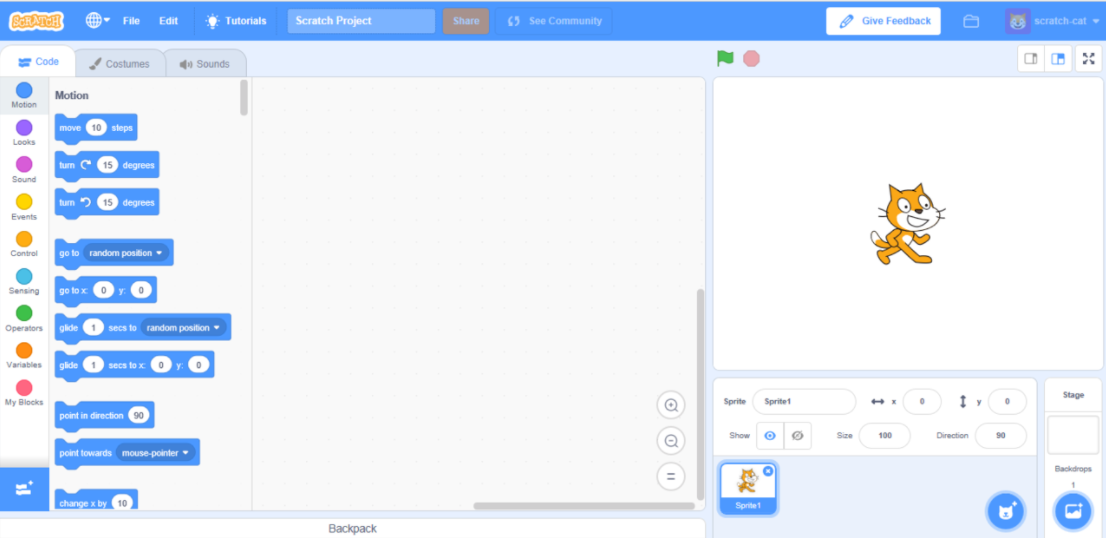
\includegraphics[scale=0.5]{scratch.PNG} & \newline

Scratch ofrece al usuario la posibilidad de programar construyendo una secuencia de código a partir de diversos bloques de acciones. El programador es capaz de construir la secuencia de código con rapidez y facilidad, ya que vada bloque incluye una secuencia de texto que explica la función que desempeña. Por ello, la secuencia de código finalmente podrá ser leída e interpretada como si de un texto se tratase. \newline

Este es el segundo lenguaje ofrecido por Kibotics para dar solución a los ejercicios. Gracias a la interfaz gráfica de la que dispone, Scratch es sin duda una de las mejores alternativas para aquellas personas que no disponen de nociones previas de programación.

\section{Blender}
Blender es un programa informático multi plataforma, es decir, compatible para distintos sistemas operativos como Windows o Linux. Las funciones pricipales que se pueden realizar con Blender son el modelado, iluminación, renderizado, animación y creación de gráficos tridimensionales. También se pueden realizar actividades relacionadas con la composición digital utilizando la técnica procesal de nodos, edición de vídeo, escultura y pintura digital. \newline

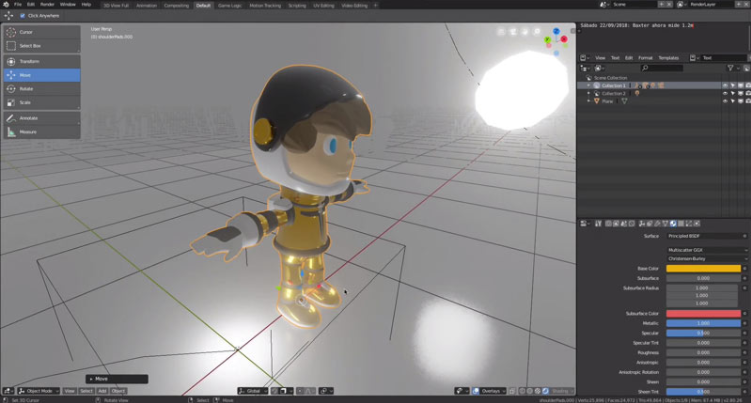
\includegraphics[scale=0.75]{blender.PNG} & \newline

Durante el presente trabajo se ha utilizado esta herramienta para modificar la rotación y apariencia de los robots de los que dispone la plataforma Kibotics. Además, Blender permite exportar los modelos en formato glTF (GL Transmission Format). glTF es un formato de archivo basado en el estandar JSON. Pemite la compresión de escenas y modelos 3D para minimizar el tiempo de ejecución de los programas en los que posteriormente se utilicen.

\section{Simulador Websim}
Websim es un simulador diseñado para el aprendizaje de conceptos básicos de programación de robots especialmente para niños. El simulador permite que os usuarios puedan programar fácilmente los movimientos de los robots, ya que simplemente tienen que acceder a la información que recoge sus sensores y enviar las órdenes precisas a los actuadores del robot. Estas órdenes se deberán programar, en Python o Scratch, en el editor que incorpora la interfaz de Websim. \newline

El simulador está diseñado basándose en el uso del entorno A-Frame. A su vez, A-Frame se sirve del motor de físicas de Cannon para materializar los movimientos de los cuerpos dinámicos en la escena. A continuación, se explican con mayor detalle ambos conceptos.

\subsection{A-Frame}
A-Frame es un marco web para crear escenas de realidad virtual. Sus principales características son las siguientes\footnote{https://aframe.io/docs/1.0.0/introduction/#features}:

\begin{itemize}
    \item Realidad vitual simplificada. Para usar A-Frame basta con colocar las etiquetas <script> y <a-scene>. A-Frame se encarga del modelado 3D y la realidad virtual, no es necesaria la instalación de ningún paquete externo.
    \item HTML declarativo. A-Frame está basado en HTML, por ello es fácil y accesible para cualquier programador, puesto que HTML es un lenguaje ampliamente conocido.
    \item Arquitectura de componente de entidad. A-Frame sigue el patrón ECS (entidad-componente-sistema). Se trata de un patrón de desarrollo de juegos basado en el principio de composición sobre herencia. De esta manera, se otorga una mayor flexibilidad en la definición de entidades ya que cada objeto de la escena se corresponde con una entidad y cada entidad, a su vez, está compuesta por uno o más componentes que contienen datos y estado de la entidad. Por tanto, una entidad puede verse modificada en tiempo de ejecución si alguno de los componentes que agrega modifica sus datos.
    \item Realidad Virtual multiplataforma. A-Frame es compatible con plataformas tan variadas como Vive, Rift, Windows Mixed Reality, Daydream, GearVR y Cardboard.
    \item Rendimiento. Las actualizaciones de A-Frame se realizan en la memoria y con poco gasto energético. A-Frame se encuentra optimizado para WebVR.
    \item Inspector visual. A-Frame cuenta con un inspecto visual integrado. Este se despliega al presionar la combinación de teclas <ctrl> + <alt> + i. El isnpector permite detectar el origen de problemas o desarrollar una mejor distribución de la escena con menos esfuerzo.
    \item Componentes. A-frame cuenta con una gran cantidad de componente con los que trabajar. Esta amplia variedad va desde componentes geométricos básicos o materiales hasta componentes como la teletransportación, la realidad aumentada o componentes personalizados por el usuario.
    \item Probado y escalable. A-Frame ha sido utilizado por empresas como Google, Disney, Samsung, Toyota o CERN, entre otras. Además, algunas de ellas, como Google, Microsoft, Oculus y Samsung han llegado a realizar contribuciones.
\end{itemize}
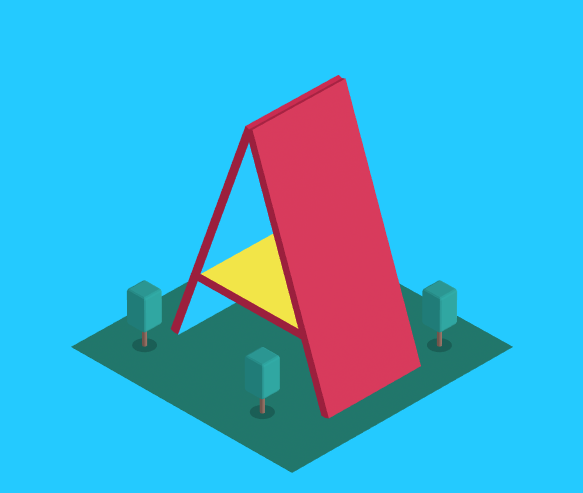
\includegraphics[scale=0.75]{a-frame.PNG} & \newline

\subsection{Sistema de físicas de A-Frame}
Las físicas de A-Frame soportan dos motores de físicas: \textit{Ammo Driver y CANNON}. Actualmente, el motor que está en uso en el del \textit{CANNON}. No obstante, ya ha sido añadido el soporte de \textit{Ammo Driver} al sistema de físicas, ya que se preveé que \textit{CANNON} acabe quedando obsoleto con el paso del tiempo. \newline

Para la instalación del sistema de físicas de A-Frame basta con incluir el siguiente script en el código html de la aplicación: 

\begin{verbatim}
<script src="//cdn.rawgit.com/donmccurdy/aframe-physics-system/v4.0.1/  
dist/aframe-physics-system.min.js"></script>
\end{verbatim}

El sistema de físicas de A-Frame cuenta con dos tipos de cuerpos: dinámicos y estáticos.

\begin{itemize}
    \item Cuerpo dinámico: aquellos objetos de la escena que presentan libertad de movimiento. Estos objetos se ven afectados por la gravedad, la fricción y las colisiones.
    \item Cuerpo estático: aquellos objetos de la escena que no necesitan modificar su posición en la misma. Son cuerpos fijos y sin animaciones. Otros cuerpos dinámicos podrán colisionar con un cuerpo estático, pero el cuerpo estático no verá modificada su posición tras la colisión.
\end{itemize}

El sistema de físicas ofrece la posibilidad de añadir una malla de colisión a un objeto de la escena. Existen mallas de colisión de diferentes formas, por lo que se debe seleccionar aquella que se ajuste mejor al objeto en cuestión. Estas son las formas que ofrece:
\begin{itemize}
    \item Automático: elige automáticamente entre las formas disponibles.
    \item Caja
    \item Cilindro
    \item Esfera
    \item Convexo
    \item Primitivas: plano, cilindro o esfera seleccionadas automáticamente en función de la primitiva A-Frame correspondiente.
\end{itemize}

Cada escena de A-Frame admite una serie de parámetros a los que se les puede modificar el valor para ajustar el mundo a las características deseadas. Si no se especifica el valor que se desea de un parámetro, este tomará el valor por defecto. Algunos de los parámetros que admite una escena son \textit{debug}, que cuando está a true muestra las mallas de colisión de los objetos de la escena o \textit{gravity, friction y restitution}, que se corresponden con la gravedad, fricción y coeficiente de restitución, respevtivmaente, del mundo que se está simulando.
\begin{table}[h!]
\centering
\begin{tabular}{|c|c|}
\hline
\textbf{Atributo}    & \textbf{Valor por defecto} \\ \hline
debug       & true              \\ \hline
gravity     & -9.8              \\ \hline
friction    & 0.01              \\ \hline
restitution & 0.3               \\ \hline
\end{tabular}
\end{table}
